\section{Selección de Dataset de Imágenes Relevantes}
Para esta práctica se ha elegido un dataset de dados vistos desde arriba. Se trata de imágenes que ya se encuentran en escala de grises y en ellas los dados se encuentran sobre fondos algo complejos por contener sombras y elementos circulares. El dataset cuenta con 2400 imágenes de las cuales 400 pertenecen a cada tipo de dado (1-6). Existen dados blancos con puntos negros y dados negros con puntos blancos.

Dataset: \url{https://github.com/tomitomi3/DiceRecognitionDatasetForML.git}

\section{Exploración visual}
Inicialmente vemos el formato que tiene un dado, y nos gustaría saber que valor del 1 al 6 tiene de manera
automática. Esto podría tener aplicación para un casino o si quisiésemos crear un bot que con computer vision tuviese una herramienta para videojuegos que incluyan dados.
\begin{center}
    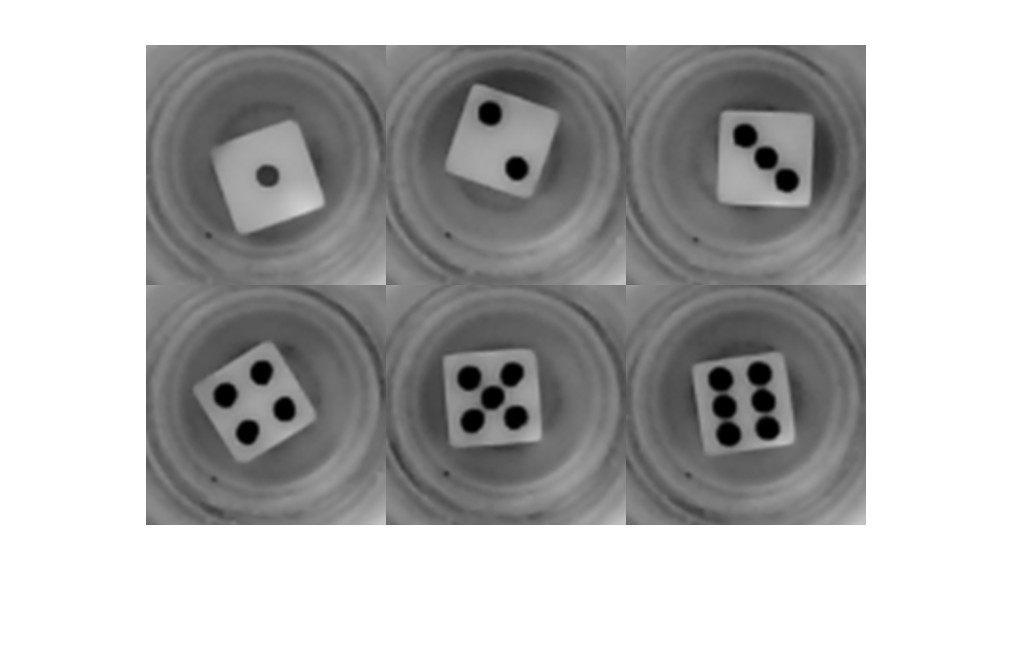
\includegraphics[width=0.5\textwidth]{ImagenesLatex/dataset.jpg}
\end{center}

Por tanto, característica a obtener: \textbf{Valor del dado}

\section{Algoritmo de Clasificación}
\subsection{Smoothing}
Se comienza con la preprocesamiento de la imagen. Se realiza un suavizado de la imagen con un filtro de media que tiene una ventana 4x4. Esto se hace para eliminar ruido de la imagen y mejorar la detección de bordes.
\begin{center}
    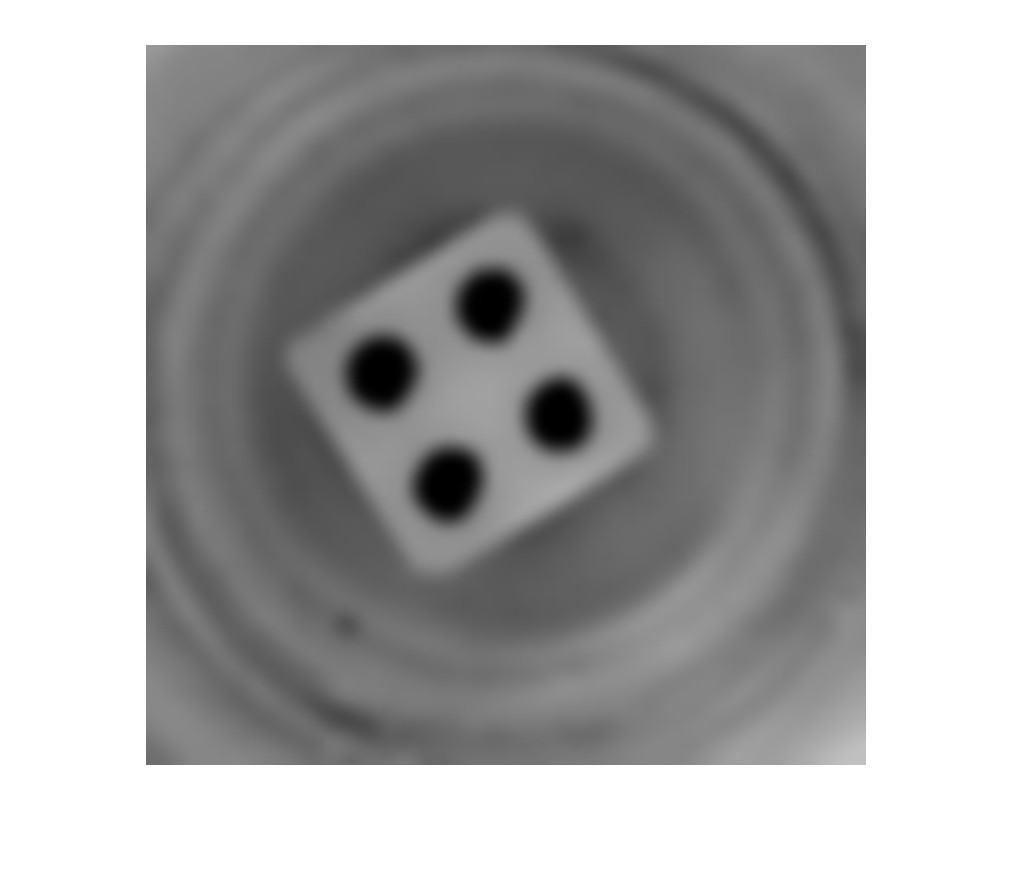
\includegraphics[width=0.4\textwidth]{ImagenesLatex/dice_smooth.jpg}
\end{center}

\subsection{Closing}
Se realiza un cierre de la imagen con un elemento estructurante con forma "disk" de radio 10. Esto se hace para eliminar los bordes de la imagen y mejorar la detección de los contornos.
\begin{center}
    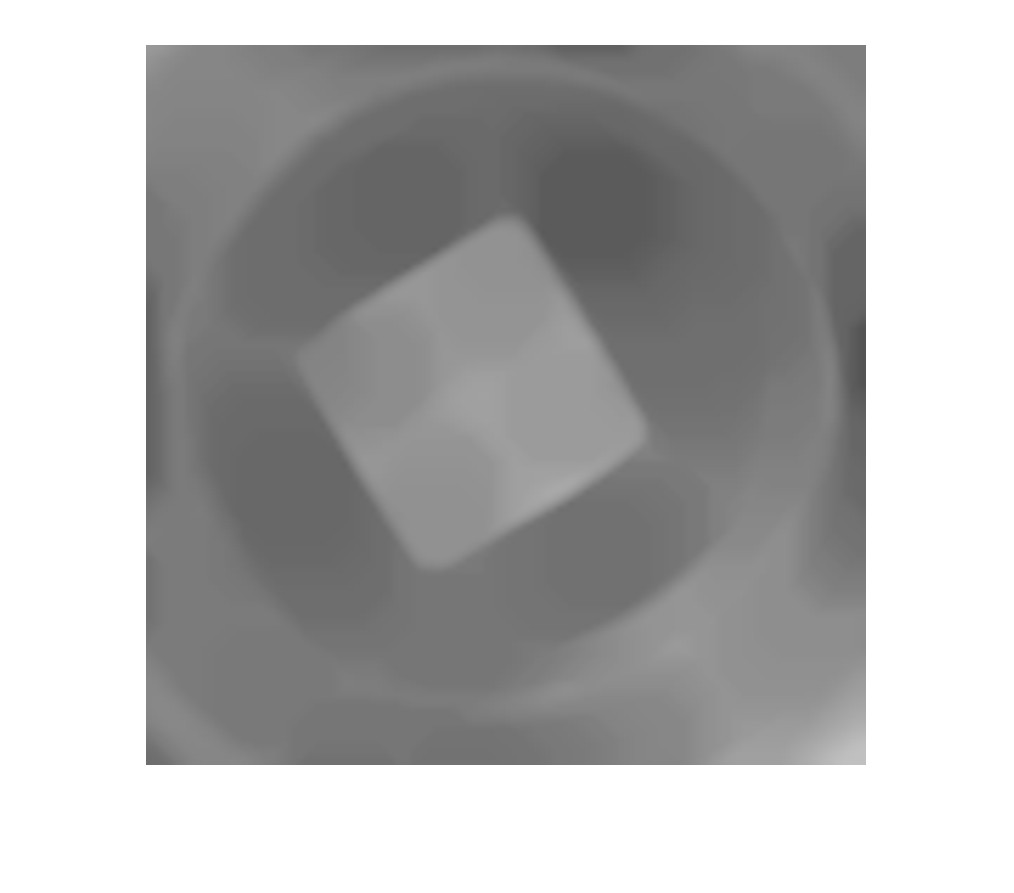
\includegraphics[width=0.4\textwidth]{ImagenesLatex/dice_close.jpg}
\end{center}

\newpage
\subsection{Adjusting}
Se aumenta el contraste de la imagen con un ajuste de contraste. Esto facilita técnicas como la creación de máscaras, aunque en nuestro caso utilizaremos la operación morfológica de blackhat.
\begin{center}
    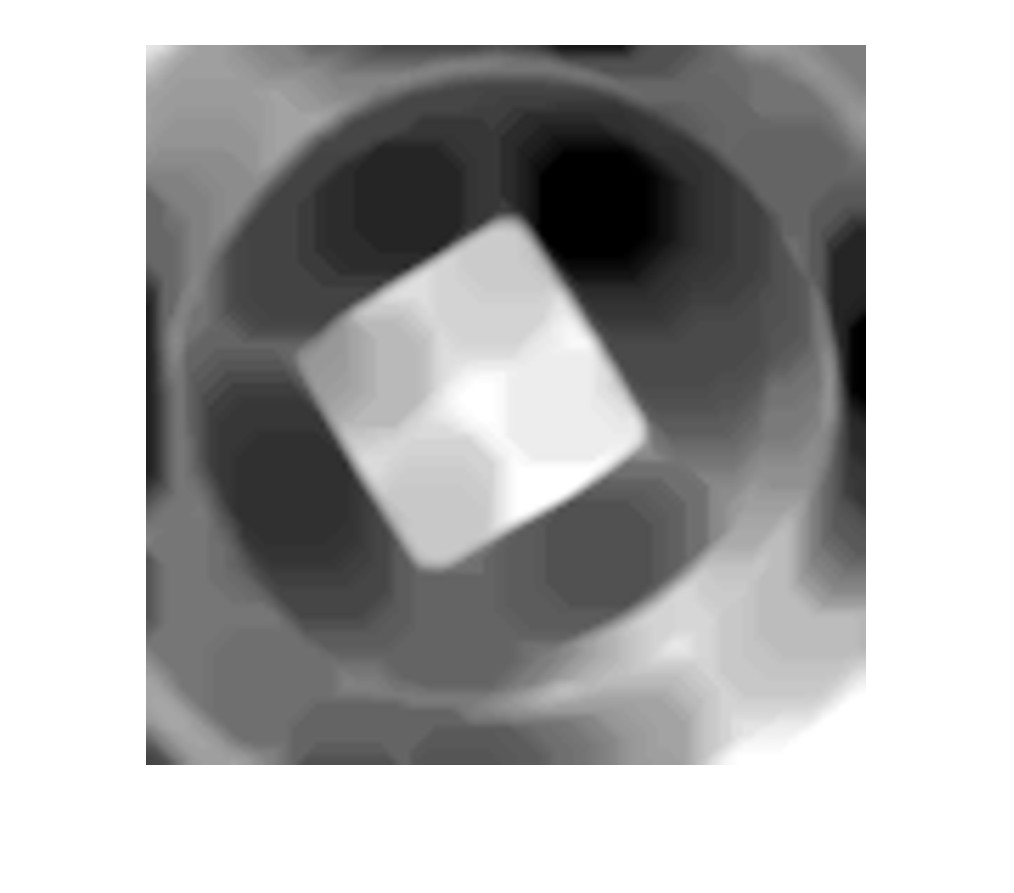
\includegraphics[width=0.4\textwidth]{ImagenesLatex/dice_adjust.jpg}
\end{center}

\subsection{Black Hat}
Se realiza una operación morfológica blackhat a partir del close obtenido anteriormente, esto nos permite eliminar el fondo y dejar solo los puntos de los dados.
\begin{center}
    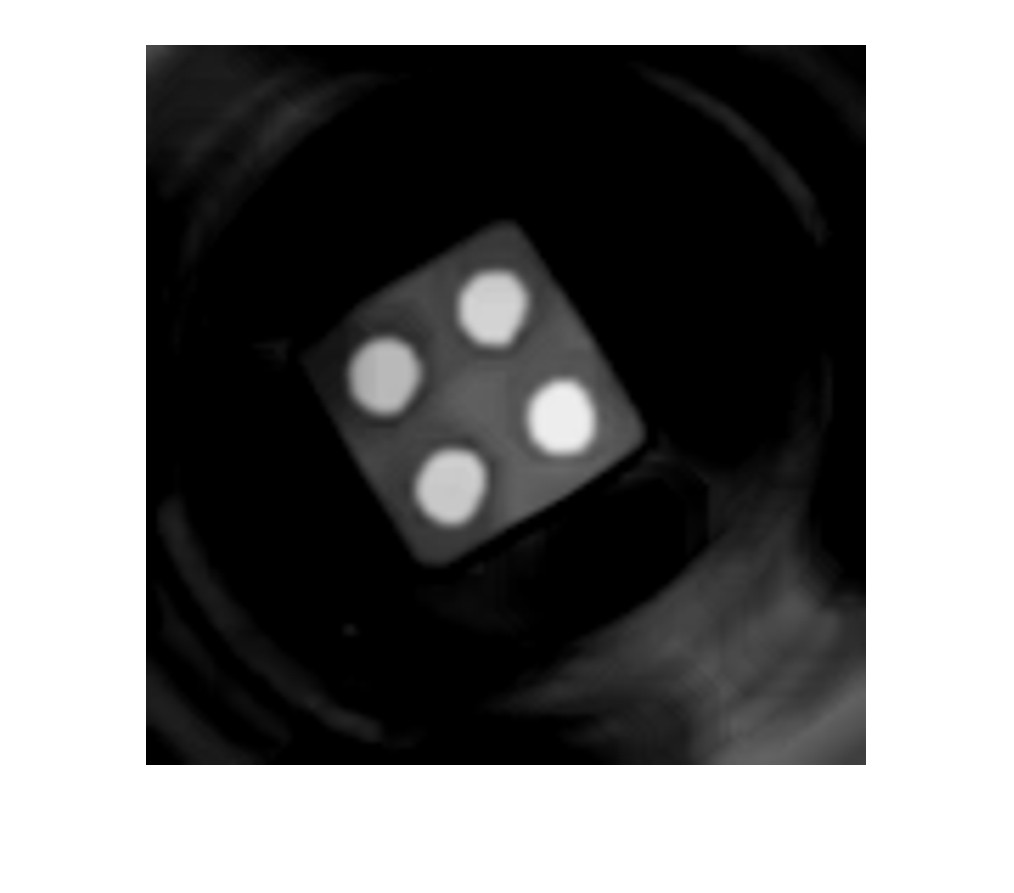
\includegraphics[width=0.4\textwidth]{ImagenesLatex/blackhat.jpg}
\end{center}

\newpage

\subsection{Thresholding}
Utilizando un umbral de 128 obtenemos una imagen binaria de los puntos de los dados.

\begin{center}
    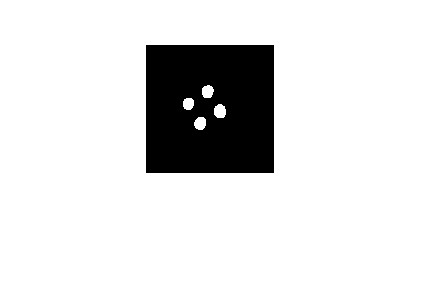
\includegraphics[width=0.9\textwidth]{ImagenesLatex/dots.jpg}
\end{center}

\subsection{Identificación de puntos}
Utilizamos la función imfindcircles de MATLAB con parámetros adecuados para identificar los puntos de los dados. Para este tipo de imágenes se buscan círculos con radios entre 6 y 12. También se reduce la sensibilidad con el objetivo de identificar puntos muy juntos que se dan en los casos de dados de valores 5 y 6. Y adicionalmente si no se detectan círculos se elige el valor 1 para el dado y si el número de círculos detectados es superior a 6 se elige el valor 6.
\begin{center}
    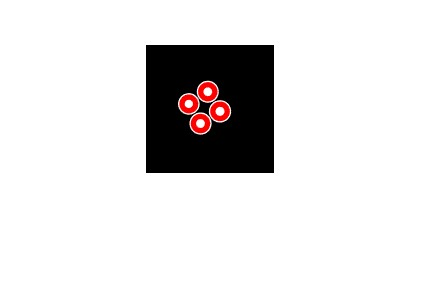
\includegraphics[width=0.9\textwidth]{ImagenesLatex/circles.jpg}
\end{center}

Obtenemos resultados bastante buenos para dados blancos.

\begin{center}
    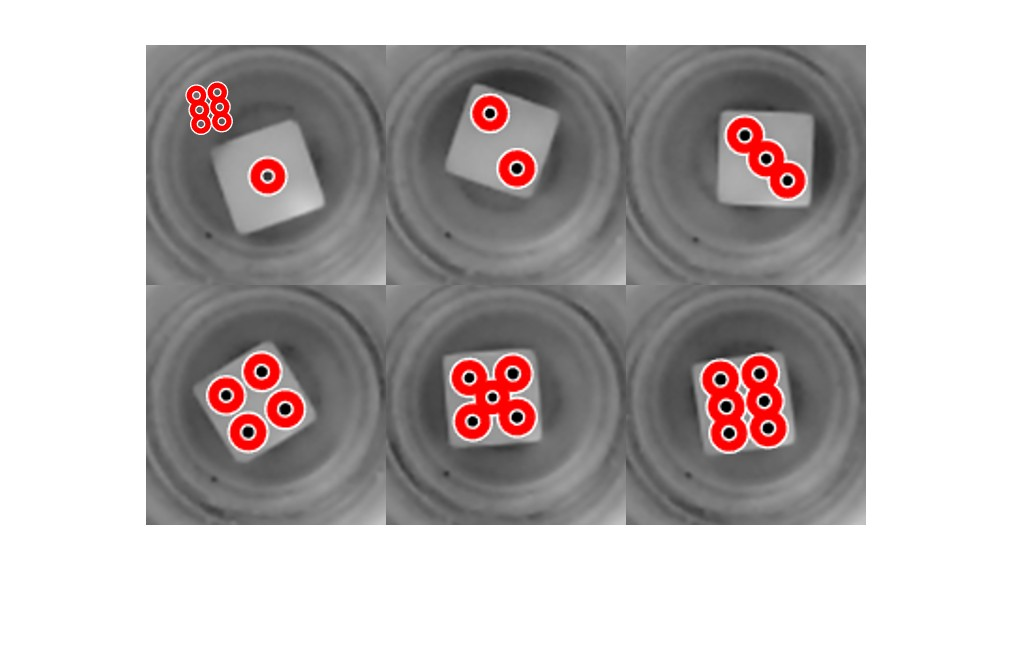
\includegraphics[width=0.9\textwidth]{ImagenesLatex/dices_circles.jpg}
\end{center}

No obstante fallamos en los dados negros.

\begin{center}
    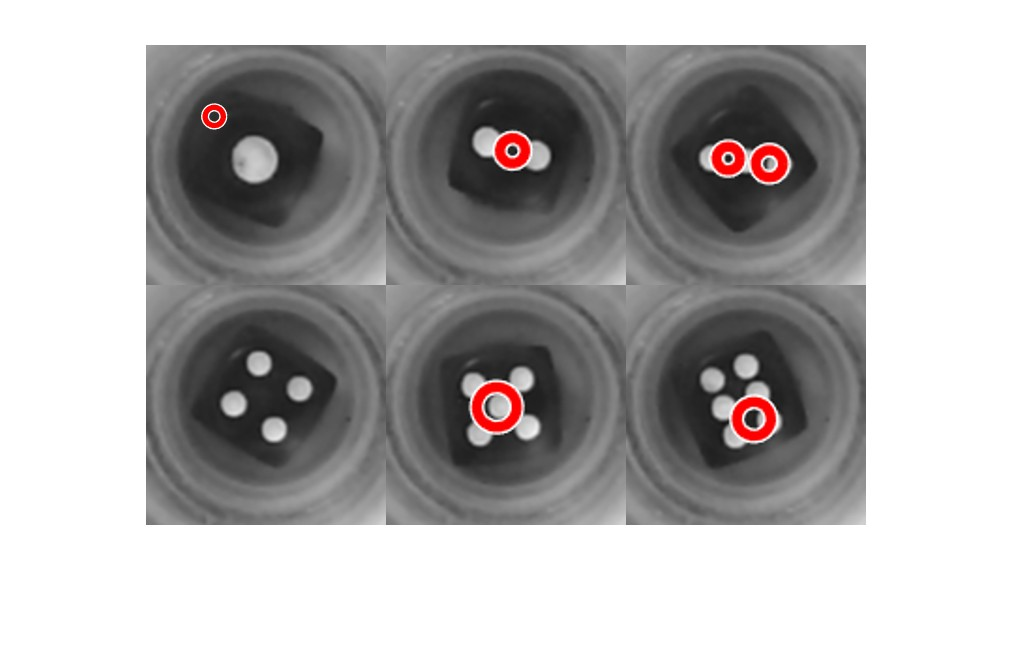
\includegraphics[width=0.9\textwidth]{ImagenesLatex/black_dice.jpg}
\end{center}

Aunque se ha conseguido obtener resultados muy buenos para los dados blancos, no es posible utilizar la misma técnica para los dados negros.

Para el total del dataset se ha propuesto un algoritmo sencillo pero funcional. La probabilidad de acertar el dado lanzando un dado es de un 16.6\% para mejorar el caso de este generador de números aleatorios, el siguiente algoritmo obtiene un 72.79\% de precisión.

\subsection{Filtro sobel}
Se trata de un filtro para la identificación de contornos, y aunque menos sofisticado que el filtro Canny obtiene resultados simples que funcionan bien para nuestro caso.

Al combinarlo con la función \textbf{imfindcircles} obtenemos resultados bastante buenos tanto para dados blancos como para dados negros.

\begin{center}
    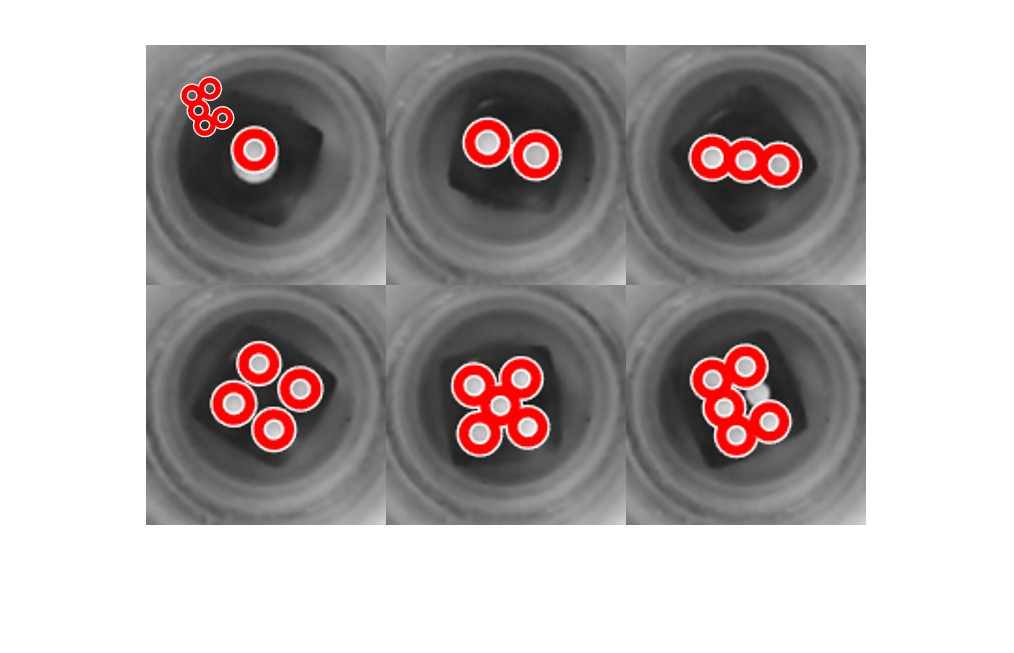
\includegraphics[width=0.9\textwidth]{ImagenesLatex/sobel_black.jpg}
\end{center}

\begin{center}
    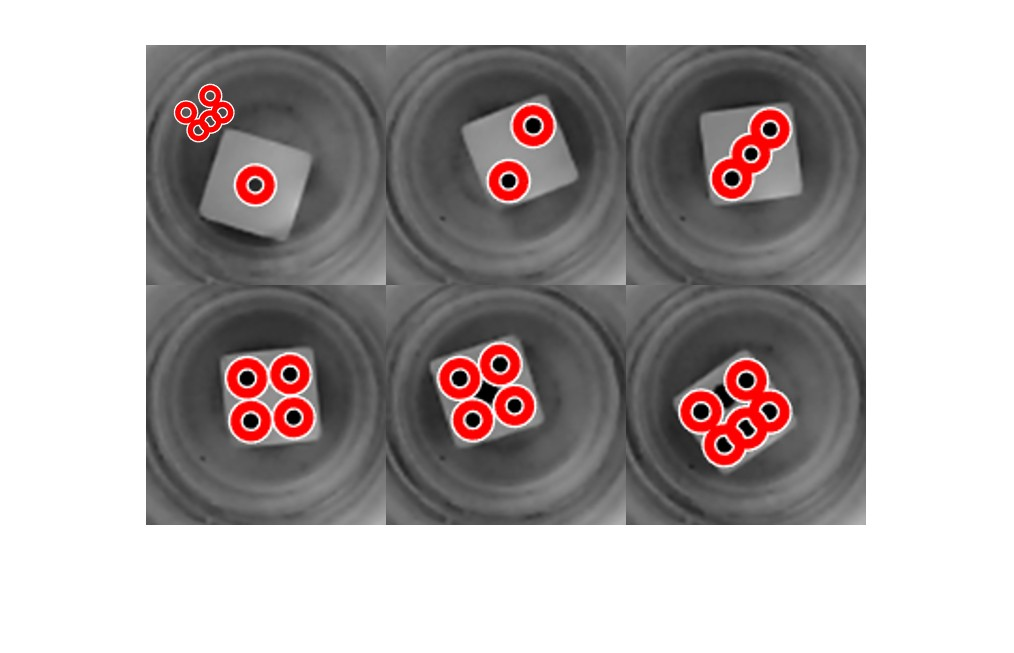
\includegraphics[width=0.9\textwidth]{ImagenesLatex/sobel_white.jpg}
\end{center}

Hemos obtenido la matriz de confusión que muestra el error cometido en el algoritmo de clasificación.

\begin{center}
    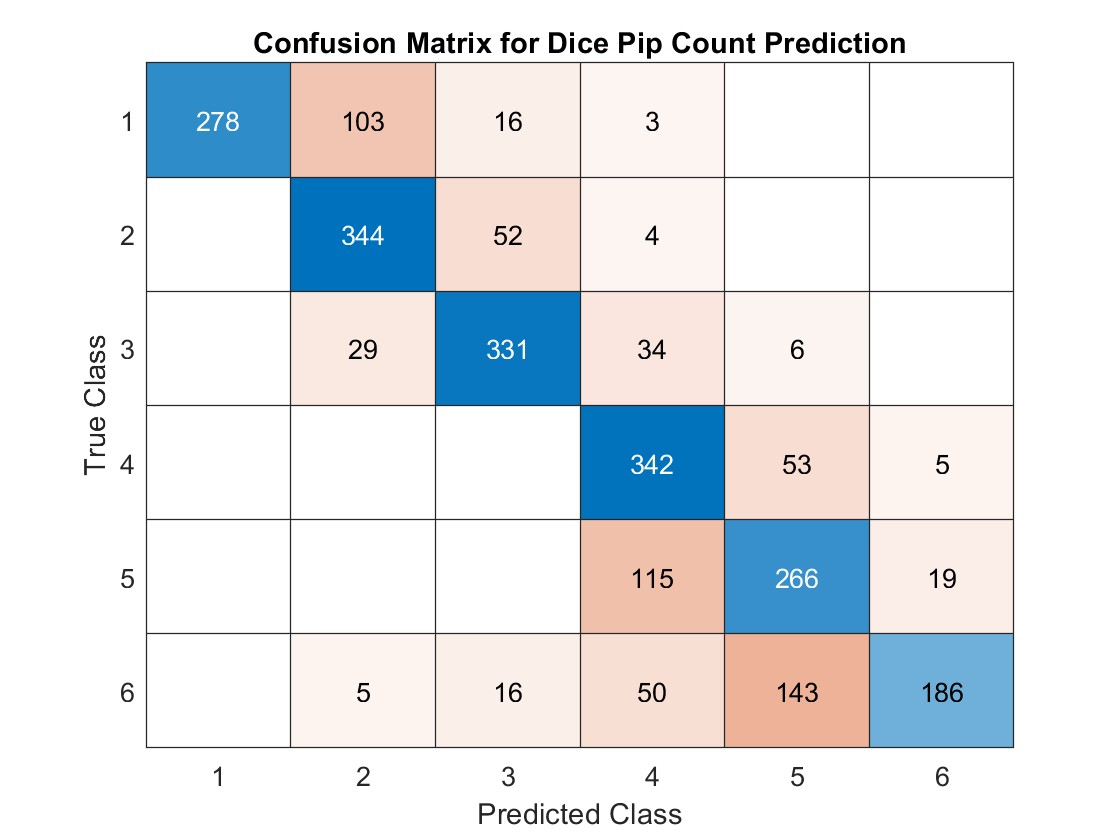
\includegraphics[width=0.9\textwidth]{ImagenesLatex/confusion.jpg}
\end{center}

Observándose una precisión del 72.79\% mejorando considerablemente el caso de utilizar un generador de números aleatorios (1/6).
